\section{现场添加指令和答辩记录}

\subsection{现场添加指令}
\subsubsection{分工情况}

在讨论分析之后,胡欣凯现场添加修改代码,共同调试修复错误。

\subsubsection{完成情况}

\begin{figure}[H]
    \centering
    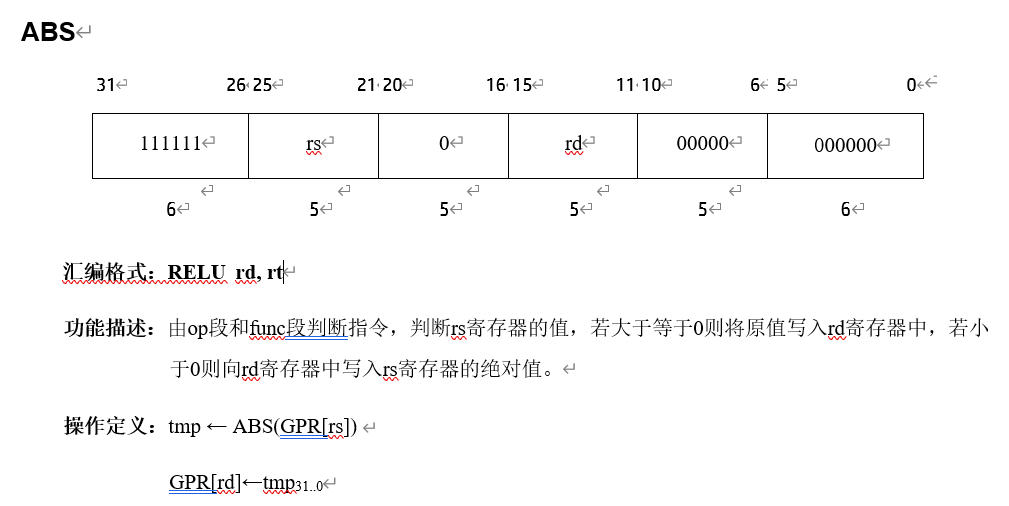
\includegraphics[width=0.8\textwidth]{image/addinst.png}
    \caption{题目}
    \label{fig:my_label}
\end{figure}

根据指令的 opcode 字段即可确定该指令,据此在 defines.vh 中定义对应的宏,并为指令分配唯一的 ALU 控制信号。

\begin{lstlisting}[language=Verilog]
//现场添加指令
`define ABS_OP 6'b111111
`define ABS_CONTROL 5'b01110
\end{lstlisting}

在 alu\_decoder.v 中,为该指令添加 ALU 控制信号 aluctrl,在 opcode 为 `ABS\_OP 时将其赋值为 `ABS\_CONTROL。

\begin{lstlisting}[language=Verilog]
assign aluctrl = 
    //现场添加指令
    opcode == `ABS_OP ? `ABS_CONTROL :

    opcode == `ANDI ? `AND_CONTROL :
    opcode == `XORI ? `XOR_CONTROL :
    opcode == `LUI ? `LUI_CONTROL :
    opcode == `ORI ? `OR_CONTROL :
    opcode == `ADDI ? `ADD_CONTROL :
    opcode == `ADDIU ? `ADDU_CONTROL :
    opcode == `SLTI ? `SLT_CONTROL :
    opcode == `SLTIU ? `SLTU_CONTROL :
    opcode == `LB ? `ADD_CONTROL :
    opcode == `LBU ? `ADD_CONTROL :
    opcode == `LH ? `ADD_CONTROL :
    opcode == `LHU ? `ADD_CONTROL :
    opcode == `LW ? `ADD_CONTROL :
    opcode == `SB ? `ADD_CONTROL :
    opcode == `SH ? `ADD_CONTROL :
    opcode == `SW ? `ADD_CONTROL :

    (opcode == `SPECIAL3_INST && rs == `MTC0) ? `MTC0_CONTROL :
    (opcode == `SPECIAL3_INST && rs == `MFC0) ? `MFC0_CONTROL :

    opcode != `R_TYPE ? `NOP_CONTROL :
    funct == `AND ? `AND_CONTROL :
    funct == `OR ? `OR_CONTROL :
    funct == `XOR ? `XOR_CONTROL :
    funct == `NOR ? `NOR_CONTROL :

    funct == `SLL ? `SLL_CONTROL :
    funct == `SRL ? `SRL_CONTROL :
    funct == `SRA ? `SRA_CONTROL :
    funct == `SLLV ? `SLLV_CONTROL :
    funct == `SRLV ? `SRLV_CONTROL :
    funct == `SRAV ? `SRAV_CONTROL :

    funct == `MFHI ? `MFHI_CONTROL :
    funct == `MFLO ? `MFLO_CONTROL :
    funct == `MTHI ? `MTHI_CONTROL :
    funct == `MTLO ? `MTLO_CONTROL :

    funct == `ADD ? `ADD_CONTROL :
    funct == `ADDU ? `ADDU_CONTROL :
    funct == `SUB ? `SUB_CONTROL :
    funct == `SUBU ? `SUBU_CONTROL :
    funct == `SLT ? `SLT_CONTROL :
    funct == `SLTU ? `SLTU_CONTROL :
    funct == `MULT ? `MULT_CONTROL :
    funct == `MULTU ? `MULTU_CONTROL :
    funct == `DIV ? `DIV_CONTROL :
    funct == `DIVU ? `DIVU_CONTROL : `NOP_CONTROL;
\end{lstlisting}

在 alu.v 中,根据 ALUCtrl 信号决定计算结果。当 ALUCtrl 为 `ABS\_CONTROL 时,输出为 SrcA 的绝对值,即如果 SrcA 是负数(根据最高位判断),输出其相反数(按位取反后加 1),否则输出 SrcA。

\begin{lstlisting}[language=Verilog]
wire [31:0] AbsA;
assign AbsA = SrcA[31] == 1'b1 ? ~SrcA + 1 : SrcA;
assign ALUOut = 
    //现场添加指令
    (ALUCtrl == `ABS_CONTROL) ? AbsA :

    //Bit-wise operations.
    (ALUCtrl == `AND_CONTROL) ? SrcA & SrcB :
    (ALUCtrl == `OR_CONTROL) ? SrcA | SrcB :
    (ALUCtrl == `XOR_CONTROL) ? SrcA ^ SrcB :
    (ALUCtrl == `NOR_CONTROL) ? ~(SrcA | SrcB) :
    (ALUCtrl == `LUI_CONTROL) ? { SrcB[15:0], 16'b0 } :
    //Shift operations.
    (ALUCtrl == `SLL_CONTROL) ? SrcB << Sa :
    (ALUCtrl == `SRL_CONTROL) ? SrcB >> Sa :
    (ALUCtrl == `SRA_CONTROL) ? {32{SrcB[31]}} << (6'b100000 - { 1'b0, Sa }) | SrcB >> Sa :
    (ALUCtrl == `SLLV_CONTROL) ? SrcB << SrcA[4:0] :
    (ALUCtrl == `SRLV_CONTROL) ? SrcB >> SrcA[4:0] :
    (ALUCtrl == `SRAV_CONTROL) ? {32{SrcB[31]}} << (6'b100000 - { 1'b0, SrcA[4:0] }) | SrcB >> SrcA[4:0] :
    //Move operations.
    (ALUCtrl == `MFHI_CONTROL) ? HiLoO[63:32] :
    (ALUCtrl == `MFLO_CONTROL) ? HiLoO[31:0] :
    //Arithmetic operations.
    (ALUCtrl == `ADD_CONTROL) ? $signed(SrcA) + $signed(SrcB) :
    (ALUCtrl == `ADDU_CONTROL) ? SrcA + SrcB :
    (ALUCtrl == `SUB_CONTROL) ? $signed(SrcA) - $signed(SrcB) :
    (ALUCtrl == `SUBU_CONTROL) ? SrcA - SrcB :
    (ALUCtrl == `SLT_CONTROL) ? ($signed(SrcA) < $signed(SrcB) ? 32'b1 : 32'b0) :
    (ALUCtrl == `SLTU_CONTROL) ? (SrcA < SrcB ? 32'b1 : 32'b0) : 
    //For MTC0: REG[rt] -> CP0[rd, sel]. REG[rt] is SrcB
    (ALUCtrl == `MTC0_CONTROL) ? SrcB :
    //For MFC0: CP0[rd, sel] -> REG[rt].
    (ALUCtrl == `MFC0_CONTROL) ? CP0Data : 32'b0;
\end{lstlisting}

在 main\_decoder.v 中,当 opcode 为 `ABS\_OP 时将以下信号置为 1:
\begin{itemize}
    \item regwrite:表示 ABS 指令需要将数据写入寄存器堆;
    \item regdst:表示 ABS 指令写寄存器堆的编号由 rd 字段确定。
\end{itemize}
并将 invalid 置为 0,以防止 RI 异常。

\begin{lstlisting}[language=Verilog]
//regdst is 1 if the instruction requires 
//to write data into registers, 
//and the destination is determined by Rd.
//Otherwise the destination is determined by Rt.
assign regdst = (
    opcode == `R_TYPE || 
    //现场添加指令
    opcode == `ABS_OP) ? 
    1'b1 : 1'b0;

//regwrite is 1 if the instruction requires 
//to write data into registers.
assign regwrite = (
    //现场添加指令
    opcode == `ABS_OP ||
    //R_TYPE writes data either to registers or HiLoReg.
    (opcode == `R_TYPE && hilowrite == 1'b0) || 
    //Arithmetic operations: 
    //write ALU output into registers.
    opcode == `ANDI || 
    opcode == `XORI || 
    opcode == `LUI ||
    opcode == `ORI || 
    opcode == `ADDI || 
    opcode == `ADDIU || 
    opcode == `SLTI || 
    opcode == `SLTIU || 
    //Jump and branch operations:
    //Write return address at $31.
    jal == 1'b1 || 
    jalr == 1'b1 || 
    bal == 1'b1 ||
    //Memory access operations: 
    //load data and write it into registers.
    opcode == `LB || 
    opcode == `LBU || 
    opcode == `LH || 
    opcode == `LHU || 
    opcode == `LW ||
    //MFC0
    cp0read == 1'b1) ? 
    1'b1 : 1'b0;

assign invalid = (
    //现场添加指令
    (opcode == `ABS_OP && rt == 5'b00000 && sa == 5'b00000 && funct == 6'b00000) ||

    (opcode == `R_TYPE && sa == 5'b00000 && funct == `AND) ||
    (opcode == `R_TYPE && sa == 5'b00000 && funct == `OR) ||
    (opcode == `R_TYPE && sa == 5'b00000 && funct == `XOR) ||
    (opcode == `R_TYPE && sa == 5'b00000 && funct == `NOR) ||
    opcode == `ANDI ||
    opcode == `XORI ||
    (opcode == `LUI && rs == 5'b00000) ||
    opcode == `ORI ||
    
    (opcode == `R_TYPE && rs == 5'b00000 && funct == `SLL) ||
    (opcode == `R_TYPE && rs == 5'b00000 && funct == `SRL) ||
    (opcode == `R_TYPE && rs == 5'b00000 && funct == `SRA) ||
    (opcode == `R_TYPE && sa == 5'b00000 && funct == `SLLV) ||
    (opcode == `R_TYPE && sa == 5'b00000 && funct == `SRLV) ||
    (opcode == `R_TYPE && sa == 5'b00000 && funct == `SRAV) ||
    
    (opcode == `R_TYPE && rs == 5'b00000 && rt == 5'b00000 && sa == 5'b00000 && funct == `MFHI) ||
    (opcode == `R_TYPE && rs == 5'b00000 && rt == 5'b00000 && sa == 5'b00000 && funct == `MFLO) ||
    (opcode == `R_TYPE && rt == 5'b00000 && rd == 5'b00000 && sa == 5'b00000 && funct == `MTHI) ||
    (opcode == `R_TYPE && rt == 5'b00000 && rd == 5'b00000 && sa == 5'b00000 && funct == `MTLO) ||
    
    (opcode == `R_TYPE && sa == 5'b00000 && funct == `ADD) ||
    (opcode == `R_TYPE && sa == 5'b00000 && funct == `ADDU) ||
    (opcode == `R_TYPE && sa == 5'b00000 && funct == `SUB) ||
    (opcode == `R_TYPE && sa == 5'b00000 && funct == `SUBU) ||
    (opcode == `R_TYPE && sa == 5'b00000 && funct == `SLT) ||
    (opcode == `R_TYPE && sa == 5'b00000 && funct == `SLTU) ||
    (opcode == `R_TYPE && rd == 5'b00000 && sa == 5'b00000 && funct == `MULT) ||
    (opcode == `R_TYPE && rd == 5'b00000 && sa == 5'b00000 && funct == `MULTU) ||
    (opcode == `R_TYPE && rd == 5'b00000 && sa == 5'b00000 && funct == `DIV) ||
    (opcode == `R_TYPE && rd == 5'b00000 && sa == 5'b00000 && funct == `DIVU) ||
    opcode == `ADDI ||
    opcode == `ADDIU ||
    opcode == `SLTI ||
    opcode == `SLTIU ||
    
    (opcode == `R_TYPE && rt == 5'b00000 && rd == 5'b00000 && sa == 5'b00000 && funct == `JR) ||
    (opcode == `R_TYPE && rt == 5'b00000 && sa == 5'b00000 && funct == `JALR) ||
    opcode == `J ||
    opcode == `JAL ||
    opcode == `BEQ ||
    (opcode == `BGTZ && rt == 5'b00000) ||
    (opcode == `BLEZ && rt == 5'b00000) ||
    opcode == `BNE ||
    (opcode == `REGIMM_INST && rt == `BLTZ) ||
    (opcode == `REGIMM_INST && rt == `BLTZAL) ||
    (opcode == `REGIMM_INST && rt == `BGEZ) ||
    (opcode == `REGIMM_INST && rt == `BGEZAL) ||

    opcode == `LB ||
    opcode == `LBU ||
    opcode == `LH ||
    opcode == `LHU ||
    opcode == `LW ||
    opcode == `SB ||
    opcode == `SH ||
    opcode == `SW ||
    
    (opcode == `R_TYPE && funct == `BREAK) ||
    (opcode == `R_TYPE && funct == `SYSCALL) ||
    
    (opcode == `SPECIAL3_INST && rs == `MTC0 && instr[10:3] == 8'b00000000) ||
    (opcode == `SPECIAL3_INST && rs == `MFC0 && instr[10:3] == 8'b00000000) ||
    instr == 32'b010000_1_0000_0000_0000_0000_000_011000) ?
    1'b0 : 1'b1;
\end{lstlisting}

按时完成现场添加指令并通过测试。

\begin{figure}[H]
    \centering
    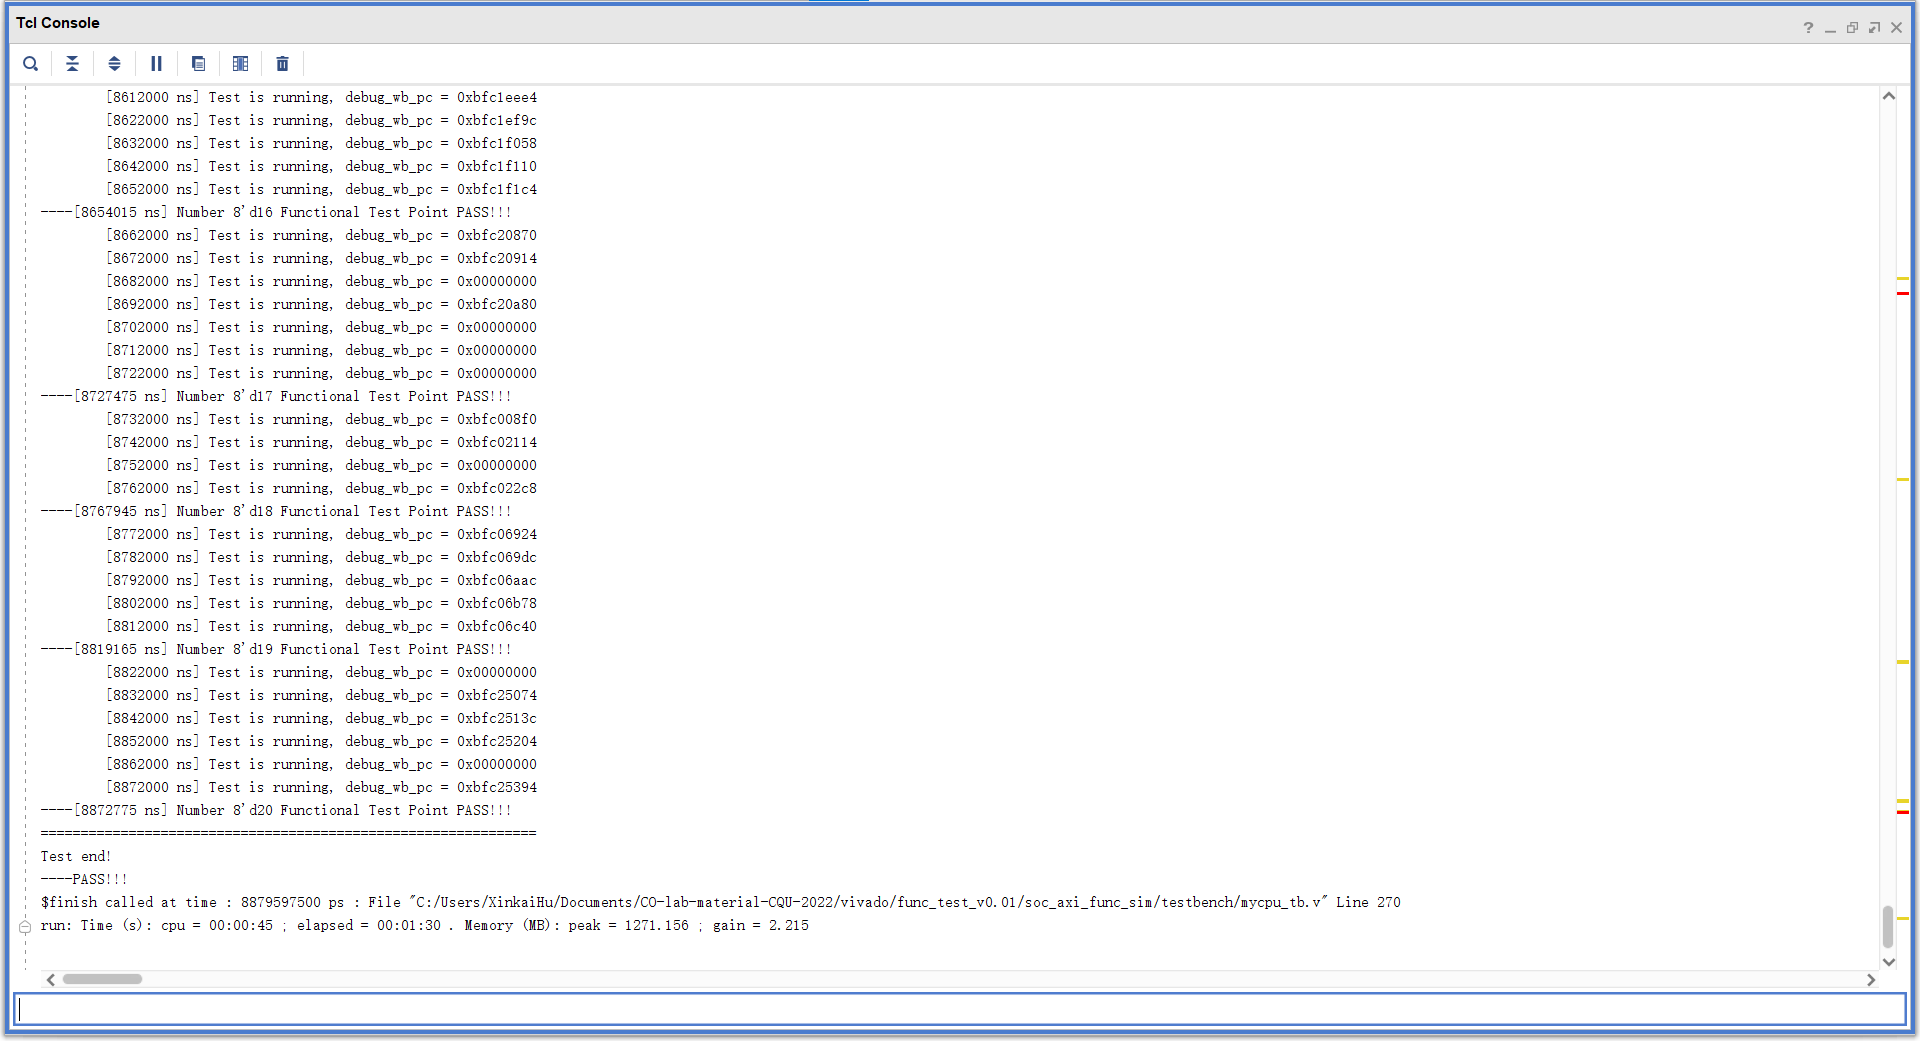
\includegraphics[width=\textwidth]{image/现场添加指令测试通过.png}
    \caption{现场添加指令测试通过}
    \label{fig:现场添加指令测试通过}
\end{figure}

\appendix

\section{Datapath代码}

\begin{lstlisting}[language=Verilog]
`timescale 1ns / 1ps

module datapath
(
    input wire clock,
    input wire reset,

    input wire [31:0] InstrF,

    input wire BranchD,
    input wire JD,
    input wire JalD,
    input wire JalrD,
    input wire JrD,

    input wire [4:0] ALUCtrlE,
    input wire ALUSrcE,
    input wire BalE,
    input wire ImmSignE,
    input wire JalE,
    input wire JalrE,
    input wire MemtoRegE,
    input wire RegDstE,
    input wire RegWriteE,

    input wire HiLoWriteM,
    input wire MemtoRegM,
    input wire [31:0] ReadDataM,
    input wire RegWriteM,
    input wire BreakM,
    input wire SyscallM,
    input wire EretM,
    input wire InvalidM,
    input wire AdESM,
    input wire AdELM,
    input wire CP0WriteM,

    input wire MemtoRegW,
    input wire RegWriteW,

    input wire i_stall,
    input wire d_stall,
    output wire stall_all,

    output wire [31:0] PCF,

    output wire [31:0] ALUOutM,
    output wire [31:0] WriteDataM,
    output wire [31:0] ExceptTypeM,

    output wire [31:0] PCW,
    output wire [4:0] WriteRegW,
    output wire [31:0] ResultW,

    output wire [31:0] InstrD,
    output wire StallF,
    output wire StallD,
    output wire StallE,
    output wire StallM,
    output wire StallW,
    output wire FlushF,
    output wire FlushD,
    output wire FlushE,
    output wire FlushM,
    output wire FlushW
);

wire [31:0] NextPCF;
wire [31:0] PCPlus4F;
wire [31:0] PCPlus8F;
wire PCExceptF;
//According to `https://co.ccslab.cn/basic/extend_57/#_8`:
//This signal should be got at IF stage
//and be used in MEM stage.
wire IsInDelaySlotF;

wire [31:0] PCPlus4D;
wire [31:0] PCPlus8D;
wire [31:0] PCJumpD;
wire [31:0] PCBranchD;
wire [4:0] RsD;
wire [4:0] RtD;
wire [4:0] RdD;
wire [4:0] SaD;
wire [15:0] ImmediateD;
wire [31:0] SignImmD;
wire [31:0] UnsignImmD;
wire [31:0] rd1D;
wire [31:0] rd2D;
wire PCSrcD;
wire [31:0] SrcAD;
wire [31:0] SrcBD;
wire PCExceptD;
wire [31:0] PCD;
wire IsInDelaySlotD;
wire [5:0] OpcodeD;
wire [5:0] FunctD;

wire [31:0] PCPlus8E;
wire [4:0] RsE;
wire [4:0] RtE;
wire [4:0] RdE;
wire [4:0] SaE;
wire [31:0] rd1E;
wire [31:0] rd2E;
wire [31:0] SignImmE;
wire [31:0] UnsignImmE;
wire [31:0] SrcAE;
wire [31:0] SrcBE;
wire [31:0] WriteDataE;
wire [4:0] WriteRegE;
wire [31:0] ALUOutE;
wire [63:0] HiLoIE;
wire [63:0] HiLoOE;
wire [63:0] DivResE;
wire DivSignedE;
wire DivStartE;
wire DivStallE;
wire [31:0] ALUOutOrPCPlus8E;
wire PCExceptE;
wire OvE;
wire [31:0] PCE;
wire IsInDelaySlotE;
wire [31:0] cp0_causeE;
wire [31:0] cp0_statusE;
wire [31:0] cp0_epcE;
wire [31:0] CP0DataE;

wire [4:0] WriteRegM;
wire [63:0] HiLoIM;
wire [63:0] HiLoOM;
wire PCExceptM;
wire OvM;
wire [31:0] PCM;
wire IsInDelaySlotM;
wire [31:0] BadAddrM;
//wire [31:0] ExceptTypeM;
wire [31:0] cp0_causeM;
wire [31:0] cp0_statusM;
wire [31:0] cp0_epcM;
wire [31:0] NewPCM;
wire [4:0] RdM;

wire [31:0] ALUOutW;
wire [31:0] ReadDataW;
//wire [4:0] WriteRegW;
//wire [31:0] ResultW;
//:USELESS
//wire [63:0] HiLoIW;
//wire [63:0] HiLoOW;
//:USELESS

wire ForwardAD;
wire ForwardBD;
wire [1:0] ForwardAE;
wire [1:0] ForwardBE;
//:ERROR
//wire [1:0] ForwardHiLoE;
//:ERROR

//If jump: next PC is jump address
//If branch: next PC is branch address
//Else next PC is PC + 4
assign NextPCF =
    ((JD | JrD | JalD | JalrD) == 1'h1) ?  PCJumpD :
    (PCSrcD == 1'h1) ? PCBranchD : PCPlus4F;
assign PCPlus4F = PCF + 32'h4;
//For bal and jal: save return address PC + 8.
assign PCPlus8F = PCF + 32'h8;
assign PCExceptF = PCF[1:0] == 2'b00 ? 1'b0 : 1'b1;
//Refer to `https://co.ccslab.cn/basic/extend_57/#_7`:
assign IsInDelaySlotF = JD | JalD | JrD | JalrD | BranchD;

assign OpcodeD = InstrD[31:26];
assign RsD = InstrD[25:21];
assign RtD = InstrD[20:16];
assign RdD = InstrD[15:11];
assign SaD = InstrD[10:6];
assign FunctD = InstrD[5:0];
assign ImmediateD = InstrD[15:0];
assign SignImmD = { {16{ImmediateD[15]}}, ImmediateD };
assign UnsignImmD = { 16'b0, ImmediateD };
assign SrcAD = (ForwardAD == 1'h1 ? ALUOutM : rd1D);
assign SrcBD = (ForwardBD == 1'h1 ? ALUOutM : rd2D);
//Branch address
assign PCBranchD = { SignImmD[29:0], 2'b00 } + PCPlus4D;
//If jr or jalr: jump address is from register rs
//If j or jal: jump address is from instruction
assign PCJumpD = ((JrD | JalrD) == 1'b1) ? SrcAD : { PCPlus4D[31:28], InstrD[25:0], 2'h0 };
//pcsrc is 1 if branch
assign PCSrcD = BranchD & (
    (OpcodeD == `BEQ && SrcAD == SrcBD) ||
    (OpcodeD == `BGTZ && SrcAD[31] == 1'b0 && SrcAD != 32'h0) ||
    (OpcodeD == `BLEZ && (SrcAD[31] == 1'b1 || SrcAD == 32'h0)) ||
    (OpcodeD == `BNE && SrcAD != SrcBD) ||
//:ERROR
//    (OpcodeD == `BLTZ && $signed(SrcAD) < 0) ||
//    (OpcodeD == `BGEZ && $signed(SrcAD) >= 0) ||
//:ERROR
    (OpcodeD == `REGIMM_INST && (RtD == `BLTZ || RtD == `BLTZAL) && SrcAD[31] == 1'b1) ||
    (OpcodeD == `REGIMM_INST && (RtD == `BGEZ || RtD == `BGEZAL) && SrcAD[31] == 1'b0) ? 
    1'b1 : 1'b0);

//If bal or jal or jalr: write PC + 8 to registers.
assign ALUOutOrPCPlus8E = (BalE | JalE | JalrE) == 1'b1 ? PCPlus8E : ALUOutE;
assign SrcAE =
    (ForwardAE == 2'h0) ? rd1E :
    (ForwardAE == 2'h1) ? ResultW :
    (ForwardAE == 2'h2) ? ALUOutM : 32'h0;
assign WriteDataE = 
    (ForwardBE == 2'h0) ? rd2E :
    (ForwardBE == 2'h1) ? ResultW :
    (ForwardBE == 2'h2) ? ALUOutM : 32'h0;
assign SrcBE = 
    (ALUSrcE == 1'h0) ? WriteDataE : 
    (ImmSignE == 1'h1) ? SignImmE : UnsignImmE;
//:ERROR
//assign HiLoOE =
//    (ForwardHiLoE == 2'h0) ? HiLoOW :
//    (ForwardHiLoE == 2'h1) ? HiLoIW : HiLoIM;
//:ERROR
//:ERROR
//assign HiLoOE = HiLoIM;
//:ERROR
assign HiLoOE = HiLoOM;
assign WriteRegE =
    ((BalE | JalE) == 1'b1) ? 5'b11111 :
    (RegDstE == 1'h1) ? RdE : RtE;

assign BadAddrM = 
    PCExceptM == 1'b1 ? PCM :
    (AdELM | AdESM) == 1'b1 ? ALUOutM : 32'b0;

assign ResultW = (MemtoRegW == 1'h1) ? ReadDataW : ALUOutW;

assign stall_all = i_stall | d_stall | DivStallE;

regfile
RegFile
(
    .clock(~clock),
    .we3(RegWriteW),
    .ra1(RsD),
    .ra2(RtD),
    .wa3(WriteRegW),
    .wd3(ResultW),
    .rd1(rd1D),
    .rd2(rd2D)
);

alu
alu
(
    .SrcA(SrcAE),
    .SrcB(SrcBE),
    .CP0Data(CP0DataE),
    .HiLoO(HiLoOE),
    .DivRes(DivResE),
    .Sa(SaE),
    .ALUCtrl(ALUCtrlE),
    .ALUOut(ALUOutE),
    .Overflow(OvE),
    .HiLoI(HiLoIE),
    .DivSigned(DivSignedE),
    .DivStart(DivStartE)
);

normal_divider
div
(
    .clock(clock),
    .reset(reset),
    .SrcA(SrcAE),
    .SrcB(SrcBE),
    .is_signed(DivSignedE),
    .start(DivStartE),
    .stall(DivStallE),
    .result(DivResE)
);

hilo_reg
HiLoReg
(
    .clk(~clock),
    .rst(reset),
    .we(HiLoWriteM),
    .hi_i(HiLoIM[63:32]),
    .lo_i(HiLoIM[31:0]),
    .hi_o(HiLoOM[63:32]),
    .lo_o(HiLoOM[31:0])
);

except
Except
(
    .PCExcept(PCExceptM),
    .RI(InvalidM),
    .Bp(BreakM),
    .Sys(SyscallM),
    .Ov(OvM),
    .AdEL(AdELM),
    .AdES(AdESM),
    .Eret(EretM),
    .cp0_status(cp0_statusM),
    .cp0_cause(cp0_causeM),
    .cp0_epc(cp0_epcM),
    .ExceptType(ExceptTypeM),
    .NewPC(NewPCM)
);

cp0_reg
CP0
(
    .clk(~clock),
    .rst(reset),
    .we_i(CP0WriteM),
    .waddr_i(RdM),
    .raddr_i(RdE),
    .data_i(ALUOutM),
    .int_i(6'b000000),
    .excepttype_i(ExceptTypeM),
    .current_inst_addr_i(PCM),
    .is_in_delayslot_i(IsInDelaySlotM),
    .bad_addr_i(BadAddrM),
    .data_o(CP0DataE),
    .status_o(cp0_statusE),
    .cause_o(cp0_causeE),
    .epc_o(cp0_epcE)
);

hazard_unit
HazardUnit
(
    .RsD(RsD),
    .RtD(RtD),
    .BranchD(BranchD),
    .JD(JD),
    .JrD(JrD),
    .RsE(RsE),
    .RtE(RtE),
    .MemtoRegE(MemtoRegE),
    .WriteRegE(WriteRegE),
    .RegWriteE(RegWriteE),
    .HiLoReadE(HiLoReadE),
    .DivStallE(DivStallE),
    .HiLoWriteM(HiLoWriteM),
    .MemtoRegM(MemtoRegM),
    .WriteRegM(WriteRegM),
    .RegWriteM(RegWriteM),
    .HiLoWriteW(HiLoWriteW),
    .WriteRegW(WriteRegW),
    .RegWriteW(RegWriteW),
    .ExceptTypeM(ExceptTypeM),

    .stall_all(stall_all),

    .StallF(StallF),
    .StallD(StallD),
    .StallE(StallE),
    .StallM(StallM),
    .StallW(StallW),
    .FlushF(FlushF),
    .FlushE(FlushE),
    .FlushD(FlushD),
    .FlushM(FlushM),
    .FlushW(FlushW),
    .ForwardAD(ForwardAD),
    .ForwardBD(ForwardBD),
    .ForwardAE(ForwardAE),
    .ForwardBE(ForwardBE)
);

flopenrc #
(32)
pc
(
    .clock(clock),
    .reset(reset),
    .enable(~StallF),
    .clear(FlushF),
    .DataReset(32'hbfc00000),
    .DataClear(NewPCM),
    .DataIn(NextPCF),
    .DataOut(PCF)
);

flopenrc #
(130)
IF_ID
(
    .clock(clock),
    .reset(reset),
    .enable(~StallD),
    .clear(FlushD),
    .DataReset(130'b0),
    .DataClear(130'b0),
    .DataIn({
        InstrF,
        PCPlus4F,
        PCPlus8F,
        PCExceptF,
        PCF,
        IsInDelaySlotF
    }),
    .DataOut({
        InstrD,
        PCPlus4D,
        PCPlus8D,
        PCExceptD,
        PCD,
        IsInDelaySlotD
    })
);

flopenrc #
(214)
ID_EX
(
    .clock(clock),
    .reset(reset),
    .enable(~StallE),
    .clear(FlushE),
    .DataReset(214'b0),
    .DataClear(214'b0),
    .DataIn({
        rd1D,
        rd2D,
        RsD,
        RtD,
        RdD,
        SignImmD,
        UnsignImmD,
        SaD,
        PCPlus8D,
        PCExceptD,
        PCD,
        IsInDelaySlotD
    }),
    .DataOut({
        rd1E,
        rd2E,
        RsE,
        RtE,
        RdE,
        SignImmE,
        UnsignImmE,
        SaE,
        PCPlus8E,
        PCExceptE,
        PCE,
        IsInDelaySlotE
    })
);

flopenrc #
(269)
EX_MEM
(
    .clock(clock),
    .reset(reset),
    .enable(~StallM),
    .clear(FlushM),
    .DataReset(269'b0),
    .DataClear(269'b0),
    .DataIn({
        ALUOutOrPCPlus8E,
        WriteDataE,
        WriteRegE,
        HiLoIE,
        PCExceptE,
        PCE,
        IsInDelaySlotE,
        OvE,
        RdE,
        cp0_causeE,
        cp0_statusE,
        cp0_epcE
    }),
    .DataOut({
        ALUOutM,
        WriteDataM,
        WriteRegM,
        HiLoIM,
        PCExceptM,
        PCM,
        IsInDelaySlotM,
        OvM,
        RdM,
        cp0_causeM,
        cp0_statusM,
        cp0_epcM
    })
);

flopenrc #
(101)
MEM_WB
(
    .clock(clock),
    .reset(reset),
    .enable(~StallW),
    .clear(FlushW),
    .DataReset(101'b0),
    .DataClear(101'b0),
    .DataIn({
        ALUOutM,
        ReadDataM,
        WriteRegM,
        PCM
    }),
    .DataOut({
        ALUOutW,
        ReadDataW,
        WriteRegW,
        PCW
    })
);

endmodule
\end{lstlisting}


\subsection{现场答辩记录}

\subsubsection{问题 1}

问题:组相联 cache 中使用的 LRU 算法的原理和实现?

回答:在 cache 中的 LRU 算法是一种 cache 块淘汰策略,当访问 cache 缺少且(在写回 cache 中)同一组 cache 块全部都是脏数据时,需要淘汰最近最少使用的 cache 块。(展示代码)在两路组相联 cache 中,当访问 cache 命中时,未被命中的那一块就被记录为最近最少访问;当有 cache 块被替换时,未被替换的那一块就被记录为最近最少访问。

\subsubsection{问题 2}

问题:HILO 寄存器在什么阶段,为什么这么实现?

回答:在我们的设计中 HILO 寄存器 EX 阶段读,MEM 阶段写。(展示数据通路图)我们复用了 ALU 的部分数据通路,在 ALU 和 HILO 寄存器之间形成了一个环路。我们类比了寄存器堆的实现思路,将 HILO 寄存器堆的时钟信号取反,通过这种方式避免新的数据前推逻辑。

\subsubsection{问题 3}
问题:CP0 在哪个阶段。

回答:我们设计的 CP0 同样是在 EX 阶段读,MEM 阶段写。(展示数据通路图)像图中展示的这样,CP0 的各个输出从 EX 阶段通过流水线传递到 MEM 阶段,并在 MEM 阶段完成异常处理。

\subsubsection{问题 4}
问题:EPC 的作用。延迟槽的作用。

回答:EPC 寄存器保存了异常处理程序执行完毕后 PC 的返回地址。这个返回地址在异常发生时会被自动写入 EPC 寄存器中。延迟槽是位于分支跳转指令后面的一条指令。位于延迟槽中的指令发生异常时,需要在异常处理程序执行结束或跳转至其前一条指令,因此写入 EPC 的值是当前 PC 减 4(即分支跳转指令所在的 PC)。

\subsubsection{问题 5}
问题:datapath 中有哪些地方需要数据前推?

回答:(展示数据通路图)在 ID 阶段需要用到 SrcAD 和 SrcBD 的指令需要前推,比如 branch 指令在 ID 阶段根据 SrcAD 和 SrcBD 判断是否需要跳转。还有在 EX 阶段需要用到 SrcAE 和 SrcBE 的指令需要前推。SrcAE 和 SrcBE 将作为 ALU 的输入完成各种运算。